El programa \textbf{Sputnik} se trataba de una serie de misiones espaciales ejecutadas por la antigua Unión Soviética a finales de los años 50 y principios de los 60 del siglo pasado. El objetivo de este programa era probar la viabilidad de los satélites artificiales alrededor de la órbita de nuestro planeta.
Como curiosidad, señalar que el origen de la palabra \textit{Sputnik} proviene del ruso y significa \textit{satélite} o \textit{compañero de viaje}.
Durante este programa se lanzaron al espacio hasta 10 satélites diferentes. Seguidamente se describirán cada uno de ellos y el impacto que esto tuvo.\\


\textbf{Sputnik 1} [\ref{s1}] fue el primer satélite artificial de la historia el cual fue lanzado el 4 de Octubre de 1957. La importancia de este satélite recae en que fue el primer intento sin fallo de poner a orbitar alrededor de nuestro planeta un satélite artificial. Fue lanzado con el lanzador R-7 y este se encargó de analizar señales de radio que utilizaba para conocer la cantidad de electrones en la ionosfera. Estuvo en actividad durante 92 días y en la actualidad se puede visitar en la oficina neoyorquina de las Naciones Unidad.\\

\begin{figure}[H]
\begin{center}
  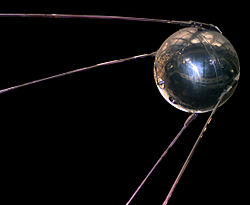
\includegraphics[width=0.5\textwidth]{./EtapaPrimeriza/imagenes/s1.jpg}
  \caption{Sputnik 1 (\href{https://es.wikipedia.org/wiki/Sputnik\_1\#/media/File:Sputnik\_asm.jpg} {Wikipedia})}
  \label{s1}
\end{center}
\end{figure}

Más tarde, se lanzó el \textbf{Sputnik 2} [\ref{s2}] el 3 de Noviembre de 1957. A diferencia del \textit{Sputnik 1}, este portaba un ser vivo en su interior. Aquí viajó la conocida \textit{Perra Laika}, y el objetivo de este lanzamiento era comprobar el efecto que causaba el medio espacial en un ser vivo. Regresó a La Tierra tras 162 días de actividad y en aquel momento de publicó que \textit{Laika} murió al regreso a nuestro planeta. Sin embargo, en 2002 fuentes rusas declararon que el animal había muerto al poco tiempo de ser lanzada a causa del estrés y el sobrecalentamiento del satélite.\\

\begin{figure}[H]
\begin{center}
  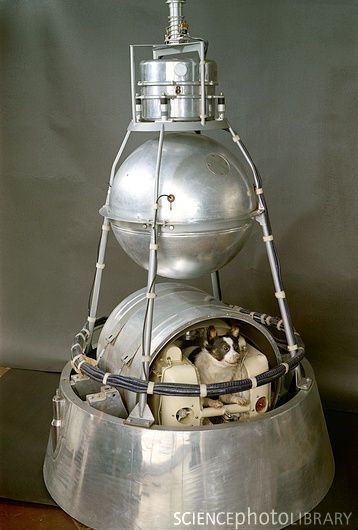
\includegraphics[width=0.3\textwidth]{./EtapaPrimeriza/imagenes/s2.jpg}
  \caption{Sputnik 2 con Laika en su interior (\href{http://www.alas-rojas.com/1-2.htm})}
  \label{s2}
\end{center}
\end{figure}

Fue el 3 de Febrero de 1958 cuando se intento lanzar el siguiente satélite, \textbf{Sputnik 3}. Esto quedó en un solo intento ya que fue fallido. Pero más tarde, se consiguió volver a lanzar esta vez ya correctamente. A pesar de que el sistema de grabación falló, transportó instrumentos para explorar la atmósfera superior y el espacio próximo.\\

\textbf{Sputnik 4} que fue lanzado el 15 de Mayo de 1960, fue el primer prototipo de nave espacial lanzada desde nuestro planeta y llevaba a bordo un maniquí de un hombre, un sistema de televisión y una cabina de soporte biológico. Pero un fallo en el sistema de guía la reubicó en una órbita más alta a la terrestre. Regresó el 5 de Septiembre de 1962, pero nada más tomar contacto con la atmósfera terrestre se desintegró. Algunas de sus piezas fueron encontradas al norte de los Estados Unidos, en Wisconsin.\\

Más tarde, el \textbf{Sputnik 5} se lanzó el 19 de agosto de 1960 y esta llevaba a bordo a los perros \textit{Belka} y \textit{Strelka} además de 40 ratones y numerosas plantas. La nave solamente permaneció en el espacio un día y todos los seres vivos regresaron con vida.\\

\textbf{Sputnik 6} fue enviado al espacio el 1 de Diciembre de 1960 con los perros \textit{Pchelka} y \textit{Mushka} junto a una serie de insectos, animales y plantas, y la cápsula no se consiguió recuperar. \\

Más tarde, el 4 de Febrero de 1961, \textbf{Sputnik 7} fue el primer intento de exploración de Venus. Sin embargo, el sistema de ignición tuvo un fallo y la sonda regresó a la órbita terrestre en lugar de tomar dirección a Venus.\\

Seguidamente, \textbf{Sputnik 8} se envió el 12 de Febrero de 1961 que transportaba la sonda Verena 1. Esta fue la primera nave espacial lanzada para sobrevolar el planeta Venus.\\

\textbf{Sputnik 9} fue una de las pruebas que tenían como finalidad iniciar los vuelos espaciales tripulados por humanos. Este completó un giro completo alrededor de nuestro planeta y volvió sin ningún problema lo que supuso un gran éxito.\\

Finalmente el \textbf{Sputnik 10}, al igual que el \textbf{Sputnik 9}, se trataba de una serie de pruebas con naves espaciales diseñadas para tripulación humana. Este portaba un perro, un astronauta ficticio y un sistema de televisión. Al igual que el anterior, se recuperó con éxito.

\begin{figure}[H]
\begin{center}
  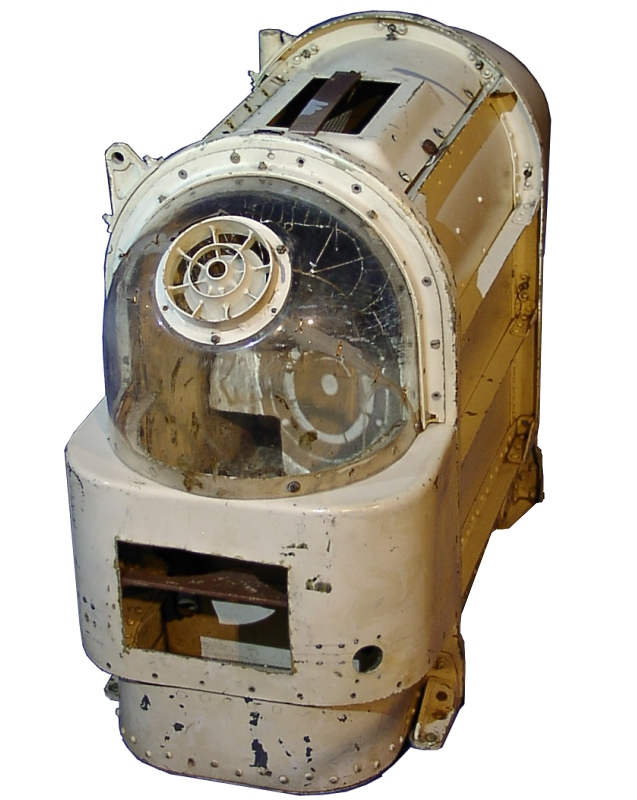
\includegraphics[width=0.3\textwidth]{./EtapaPrimeriza/imagenes/s10.jpg}
  \caption{Sputnik 10 (\href{https://es.wikipedia.org/wiki/Sputnik\_10\#/media/File:Russian\_space\_dog\_box.jpg} {Wikipedia})}
  \label{s2}
\end{center}
\end{figure}
